% !TEX root =  ../master.tex
\chapter{Nutzerhandbuch}\label{cha:Nutzerhandbuch}

Startet ein Nutzer die Anwendung, so wird er zu Beginn nach einem Token gefragt. Dieser Token ist der für die Kommunikation mit der Börse benötigte API-Token und gewährleistet, dass mit der Börse nur autorisierte Nutzer interagieren können. In unserer Anwendung wurde auf ein Login verzichtet, da bereits durch die Eingabe des API-Tokens gewährleistet wird, dass nur berechtigte Personen Simulationen starten können. 
\begin{figure}[ht]
	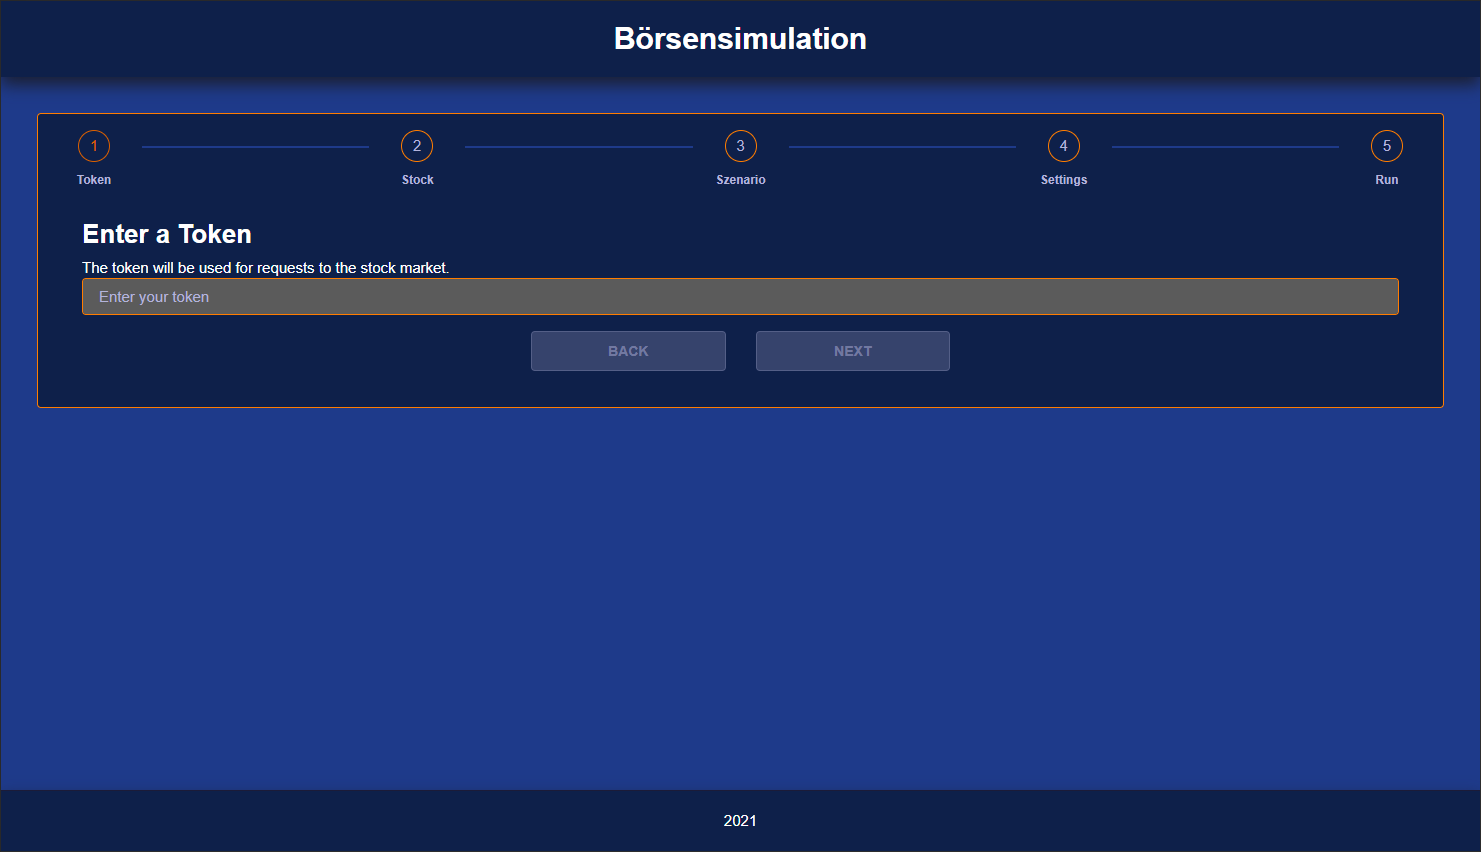
\includegraphics[width=\textwidth]{img/Token.png}
	\centering
	\caption{Start der Anwendung}
	\label{fig:token}
\end{figure}

Das Überspringen dieses Schrittes ist wie in der Abbildung ersichtlich nicht möglich, da der Button \enquote{next} erst aktiviert wird, wenn ein Token eingegeben wurde. Dies wird aus \autoref{fig:token} und Abbildung \autoref{fig:tokeninput} ersichtlich. Zudem bietet das gewählte Verfahren den Vorteil, dass der API-Token nirgends in der Simulation gespeichert werden muss. So kann dieser auch nicht durch Dritte ausgelesen werden.
\begin{figure}[ht]
	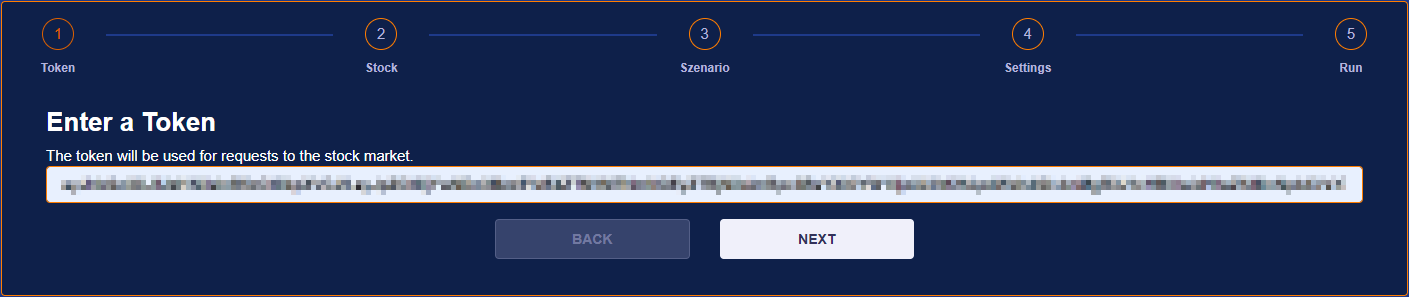
\includegraphics[width=\textwidth]{img/TokenInput.png}
	\centering
	\caption{Eingabe eines Tokens}
	\label{fig:tokeninput}
\end{figure}

Im nächsten Schritt (\autoref{fig:stock}) wählt der Nutzer eines der zur Verfügung stehenden Wertpapiere aus, für das er eine Simulation starten möchte. Hier stehen alle Wertpapiere zur Auswahl, die an der Börse gehandelt werden. Nimmt die Börse weitere Wertpapiere in den Handel auf, so sind diese sofort in dieser Liste aufgenommen.
\begin{figure}[ht]
	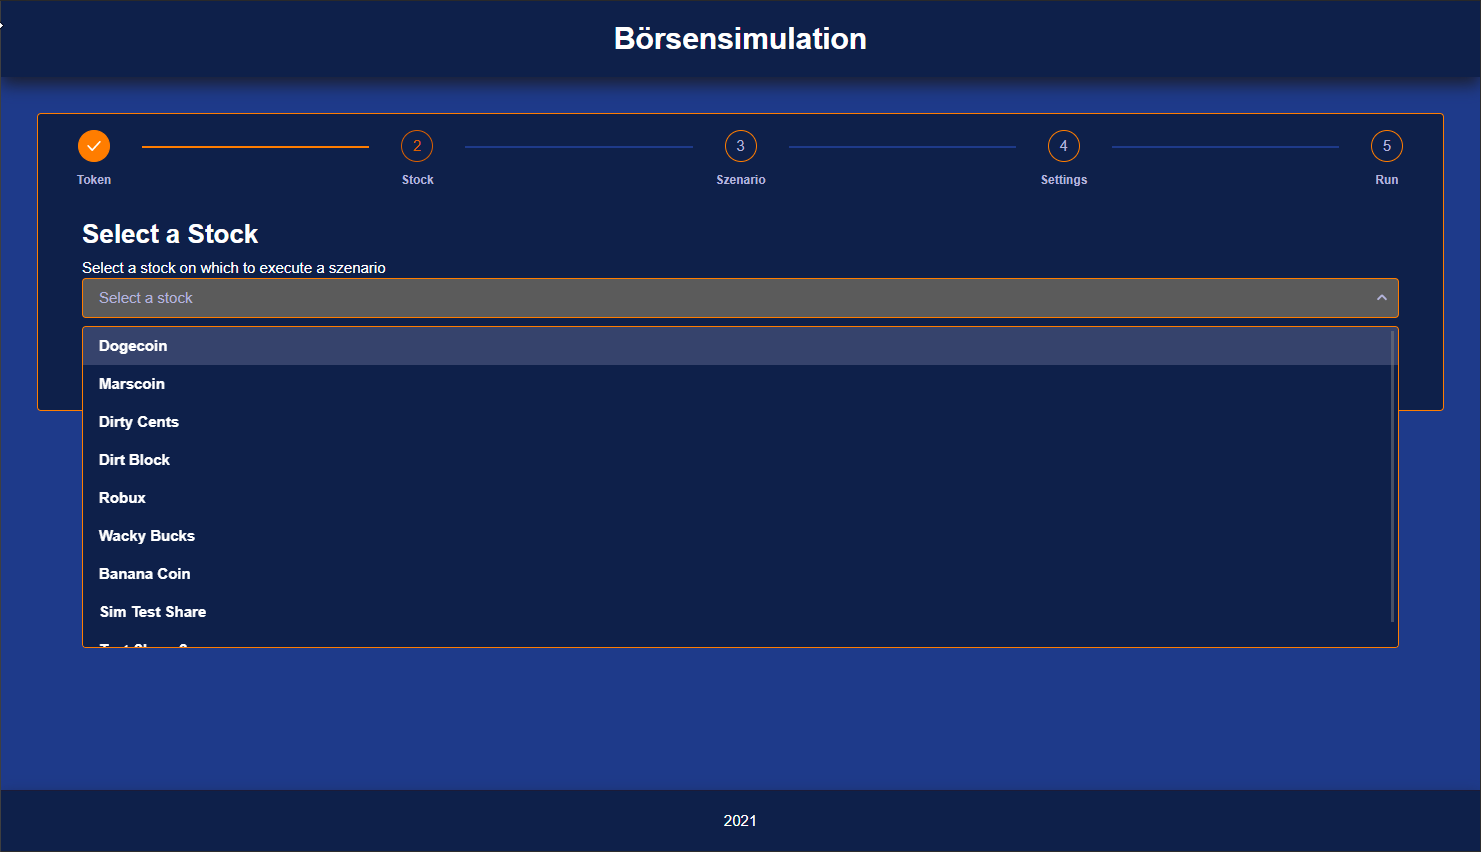
\includegraphics[width=\textwidth]{img/Stock.png}
	\centering
	\caption{Auswahl eines Wertpapiers}
	\label{fig:stock}
\end{figure}

Mit dem Bestätigen des \enquote{next} Buttons, gelangt der Nutzer zur Auswahl der Szenarien. Aktuell stehen dabei folgende Szenarien zur Verfügung:

\begin{itemize}
	\item Normaler Handelstag
	\item Positive Nachricht
	\item Geringes gehandeltes Volumen
	\item Kursabsturz durch Übernahme
	\item Hohes gehandeltes Volumen
\end{itemize}

Bei der Auswahl eines dieser Szenarien, wird darunter das simulierte Marktgeschehen dieses Szenarios angezeigt (\autoref{fig:szenario}). Die Preise werden dabei als Delta aufgelistet, da sie sich an die Kurswerte der einzelnen Wertpapiere anpassen und nicht die Preise auf ein gleiches Niveau drücken. Anschließend muss auch hier mit \enquote{next} bestätigt oder mit \enquote{back} zur Auswahl eines Wertpapieres zurückgekehrt werden. 
\begin{figure}[ht]
	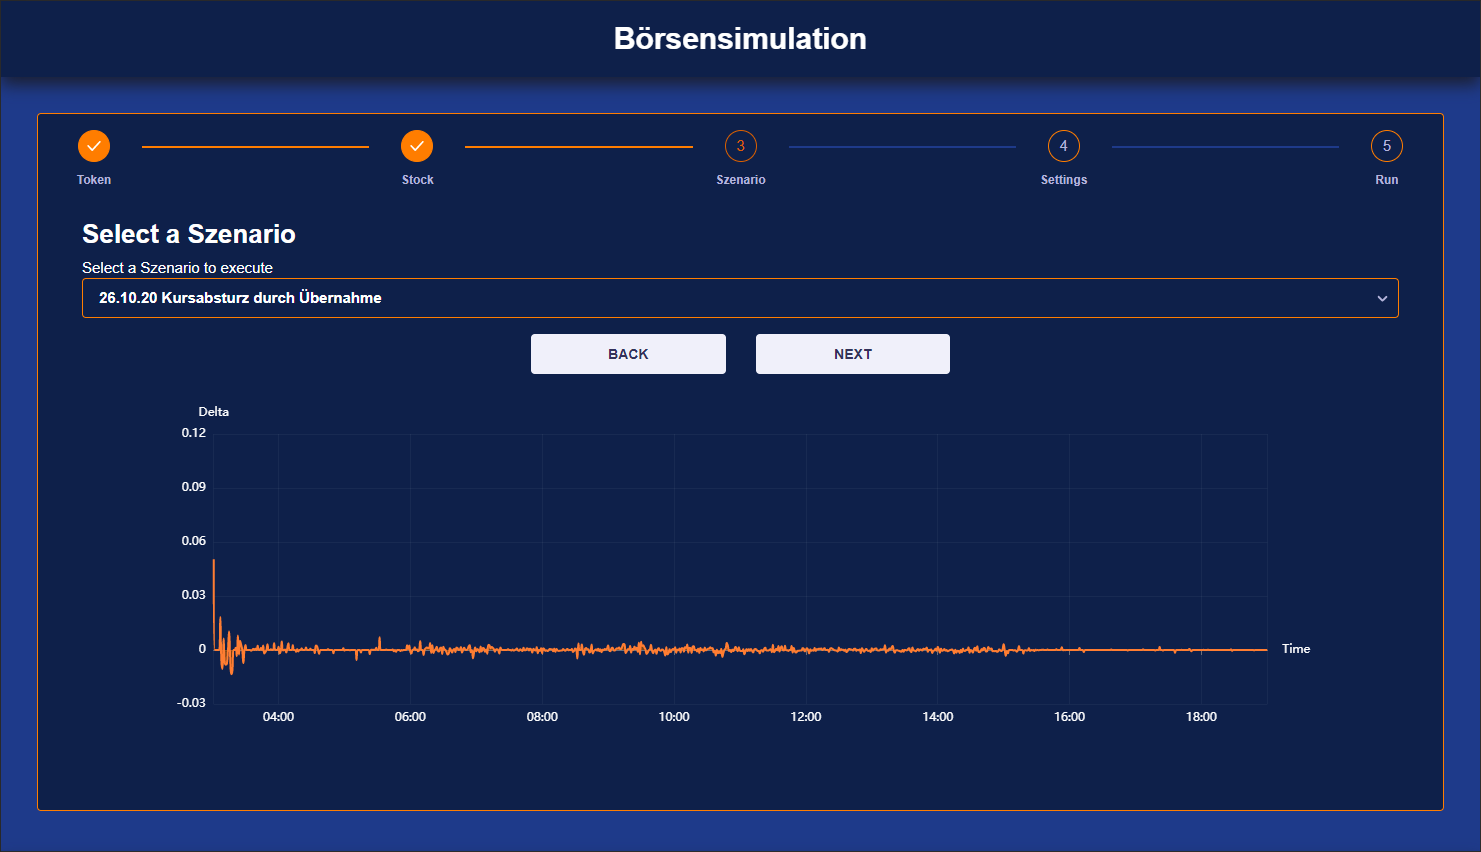
\includegraphics[width=\textwidth]{img/Szenario.png}
	\centering
	\caption{Auswahl eines Szenarios}
	\label{fig:szenario}
\end{figure}

Der Speedmultiplikator (\autoref{fig:settings}) definiert den Beschleunigungsfaktor, der bestimmt, wie viel schneller ein Szenario im Vergleich zur Echtzeit ablaufen soll. Aus Performance Gründen empfehlen wir diesen nicht über 10 und maximal 15 zu setzen, da es ansonsten zu Performance Einschränkungen der Börse kommen kann.
Dies würde alle weiteren Broker beeinflussen.
\begin{figure}[ht]
	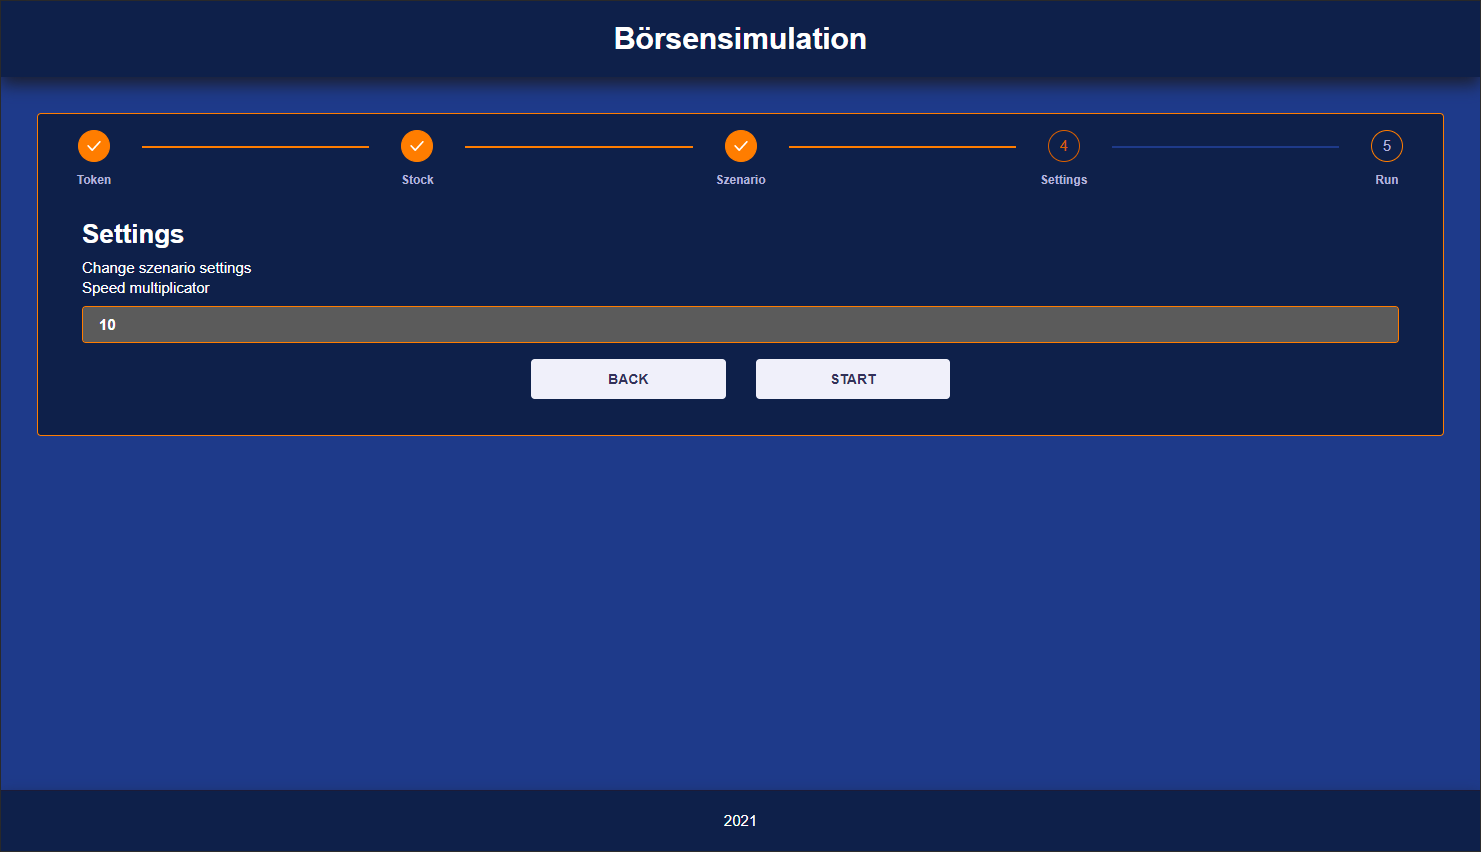
\includegraphics[width=\textwidth]{img/Settings.png}
	\centering
	\caption{Auswahl der Settings}
	\label{fig:settings}
\end{figure}

In \autoref{fig:run} ist die Ansicht dargestellt, die während der Szenarioausführung angezeigt wird. Der Balken mit der Inschrift \enquote{Running}, zeigt den Fortschritt des ausgewählten Szenarios. Über den \enquote{Stop} Button kann das Szenario jederzeit wieder gestoppt werden. Die Wirkung des Szenarios und das Testen von eigenen Strategien kann nun mit den durch die Broker und die Börse bereitgestellten Daten und Tools bewertet werden. 
\begin{figure}[ht]
	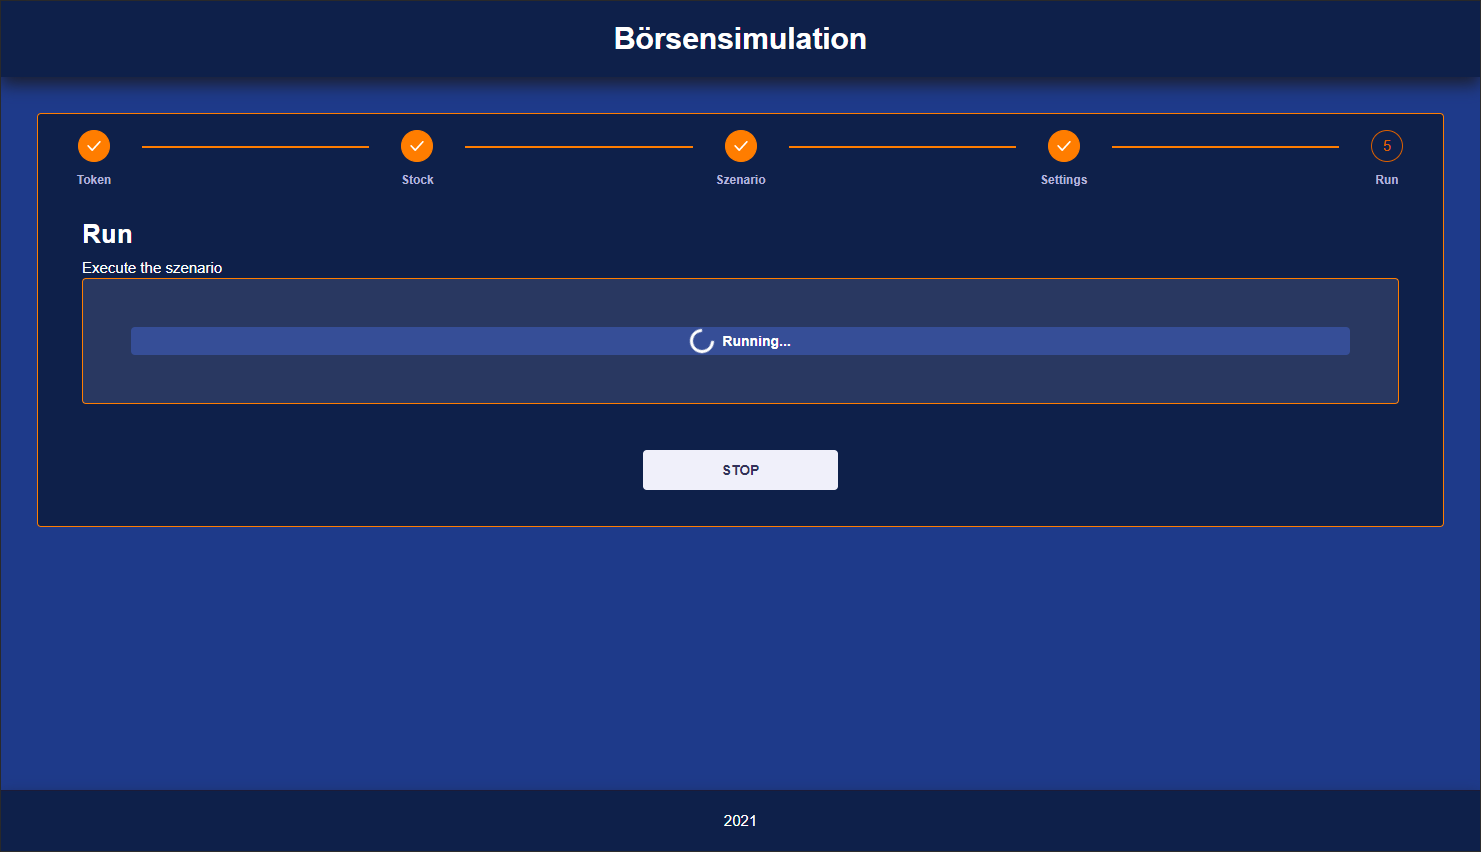
\includegraphics[width=\textwidth]{img/Run.png}
	\centering
	\caption{Laufendes Szenario}
	\label{fig:run}
\end{figure}